\section{Energy Visualization}
\label{app:energy_visualization}

Figure~\ref{fig:energy_landscape} shows the t-SNE visualization for learned $\phi(s,a)$. On locomotion tasks, e.g., Metaworld(Reach), the trajectory of latent space is smooth, while in manipulation tasks Air Hockey, the trajectory jumps whenever the interaction happens. This result supports our analysis of mode-switching challenge of CRL.

\begin{figure}
    \centering
    \vspace{-1em}
    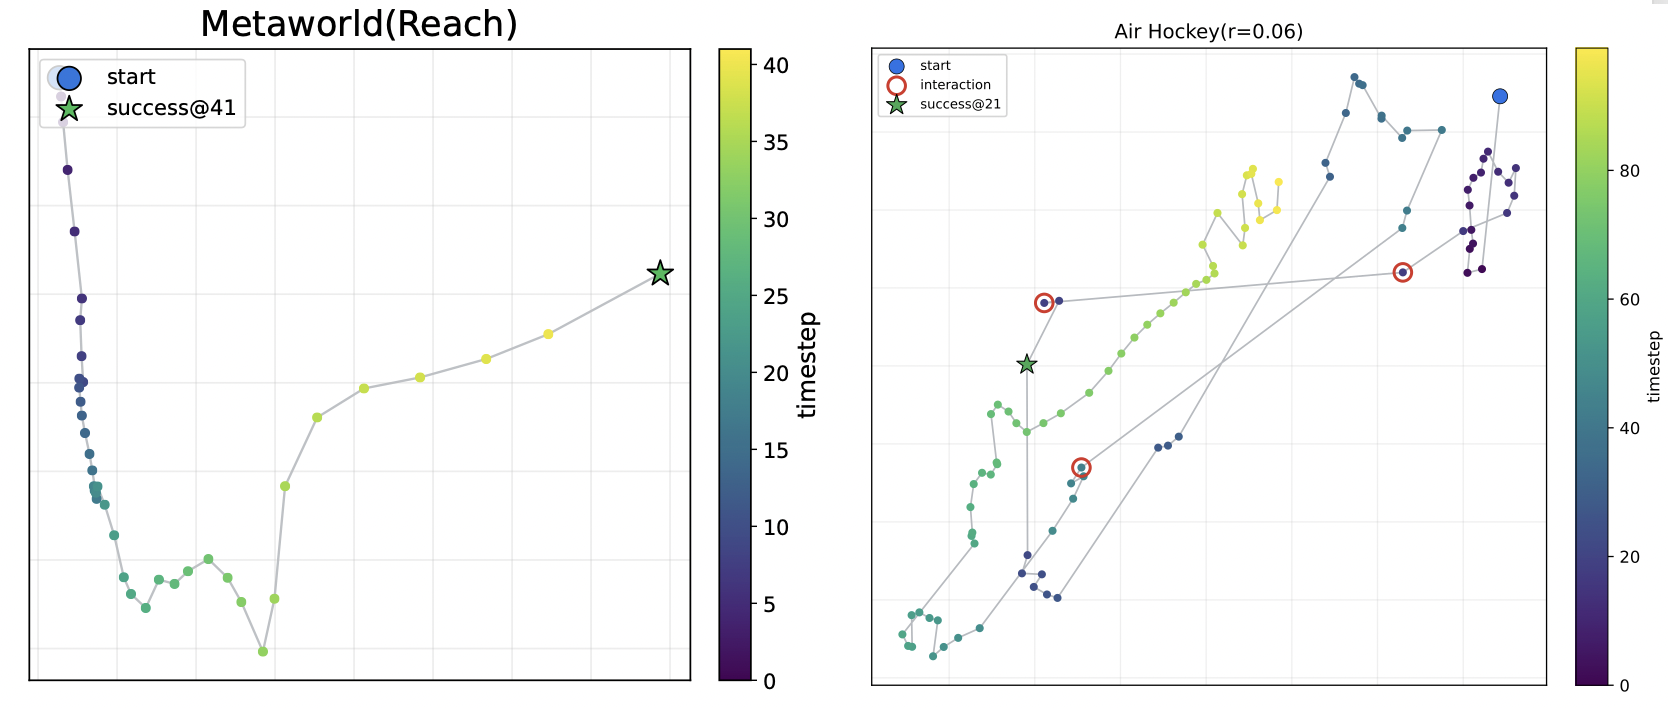
\includegraphics[width=0.98\textwidth]{figure/energy_landscape/energy.png}
    \caption{t-SNE visualization of $\phi(s,a)$ of SGCRL. Left: Metaworld(reach) Right: Air Hockey Simulator. Red circle indicates interactions. Star indicates success.
    }
    \label{fig:energy_landscape}
    \vspace{-1em}
\end{figure}

